Approximation algorithms can obtain significant benefits from using customized
scheduling policies since they follow important statistical properties and thus
can trade correctness for faster convergence. An example of such algorithm is
the Loopy Belief Propagation (LBP)~\cite{Murphy99loopybelief}. LBP is an
approximate inference algorithm used in graphical models with cycles which
employs a sum-product message passing algorithm where nodes exchange messages
with their immediate neighbors and apply some computations to the messages
received.

\begin{figure}[h]
   \begin{center}
      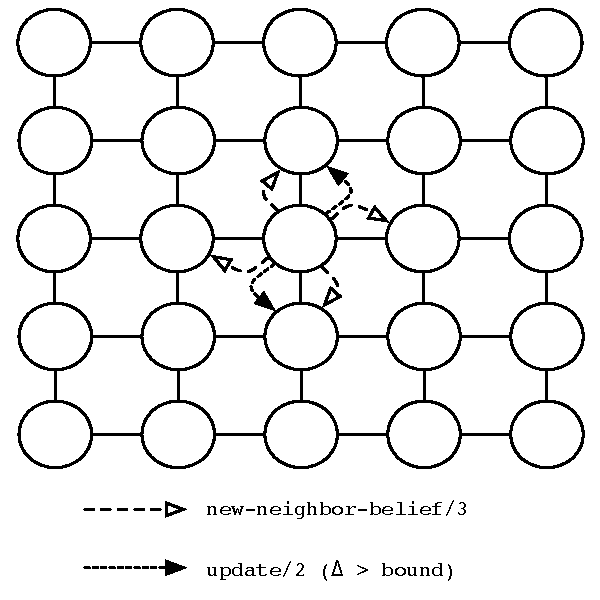
\includegraphics[width=0.3\textwidth]{figures/bp/bp.pdf}
   \end{center}

   \caption{LBP communication patterns. \code{new-neighbor-belief} facts are
   sent to the neighborhood when the node's belief value is updated. If the new
   value sent to the neighbor differs significantly from the value sent before
   the current the round, then an \code{update} fact is also sent (to the node
   above and below in this case).}

\label{fig:coordination:bp}
\end{figure}

LBP is an algorithm that maps very well to the graph-based model of LM. The
original algorithm computes the belief of all nodes using several iterations
with synchronization between iterations. However, it is possible to avoid the
synchronization step, if we take advantage of the fact that LBP will converge
even when using an asynchronous approach. So, instead of computing the belief
iteratively, we keep track of all messages sent/received (and overwrite them
when we receive a new one) and recompute the belief asynchronously.
Figure~\ref{fig:coordination:bp} presents the communication patterns of the
program, while Fig.~\ref{code:coordination:bp} presents the LM code for the
asynchronous version of LBP.

\begin{figure}[ht]
\begin{Verbatim}[numbers=left, fontsize=\codesize, commandchars=\*\#\&]
type list float belief.*hfill// Type declaration.

type potential(node, belief).*hfill// Predicate declaration
type edge(node, node).
type linear neighbor-belief(node, node, belief).
type linear new-neighbor-belief(node, node, belief).
type linear sent-neighbor-belief(node, node, belief).
type linear check-residual(node, float, node).
type linear belief(node, belief).
type linear update-messages(node, belief).
type linear update(node).

neighbor-belief(A, B, Belief),*label#line:coord:bp_first1&*hfill// Rule 1: update neighbor belief value
new-neighbor-belief(A, B, NewBelief)
   -o neighbor-belief(A, B, NewBelief).*label#line:coord:bp_first2&

check-residual(A, Residual, B),*label#line:coord:bp_check1&*hfill// Rule 2: check residual
Residual > bound
   -o update(B).

check-residual(A, _, _) -o 1.*label#line:coord:bp_check2&*hfill// Rule 3: check residual

update-messages(A, NewBelief),*hfill// Rule 4: compute belief to be sent to a neighbor node*label#line:coord:bp_iterate1&
   -o {B, OldIn, OldOut, Cavity, Convolved, OutMessage, Residual |
         !edge(A, B),
         neighbor-belief(A, B, OldIn),
         sent-neighbor-belief(A, B, OldOut),
         Cavity = normalize(divide(NewBelief, OldIn)),
         Convolved = normalize(convolve(global-potential, Cavity)),
         OutMessage = damp(Convolved, OldOut, damping)
         Residual = residual(OutMessage, OldOut)
         -o check-residual(A, Residual, B),
            new-neighbor-belief(B, A, OutMessage),
            neighbor-belief(A, B, OldIn),
            sent-neighbor-belief(A, B, OutMessage)}.*label#line:coord:bp_iterate2&

*label#line:coord:bp_last1&
update(A), update(A) -o update(A).*label#line:coord:bp_update&*hfill// Rule 5: prune redundant update operations

update(A),*hfill// Rule 6: initiate update operation*label#line:coord:bp_update1&
!potential(A, Potential),
belief(A, MyBelief)
   -o [sum Potential => Belief; B, Belief |*label#line:coord:bp_agg1&
         neighbor-belief(A, B, Belief) -o
         neighbor-belief(A, B, Belief) ->
         Normalized = normalizestruct(Belief),
         update-messages(A, Normalized), belief(A, Normalized)].*label#line:coord:bp_last2&*label#line:coord:bp_update2&*label#line:coord:bp_agg2&
\end{Verbatim}

\caption{LM code for the asynchronous version of the Loopy Belief Propagation
problem.}

\label{code:coordination:bp}
\end{figure}

\clearpage

Belief values are arrays of floats and are represented by \code{belief/2} facts.
The first rule (lines~\ref{line:coord:bp_first1}-\ref{line:coord:bp_first2})
updates a given neighbor belief whenever a new belief value is received. This is
the highest priority rule since we want to update the neighbor beliefs before
doing anything else. In order to store the belief values of the neighbor nodes,
we use \code{neighbor-belief/3} facts, where the second argument is the neighbor
address and the third argument is the belief value.

The last two rules (lines~\ref{line:coord:bp_last1}-\ref{line:coord:bp_last2})
update the belief value of a node. An \code{update} fact starts the process.
The first rule (line~\ref{line:coord:bp_update}) simply removes redundant
\code{update} facts and the second rule
(lines~\ref{line:coord:bp_update1}-\ref{line:coord:bp_update2}) performs the
belief update by aggregating all the neighbor belief values. The aggregate in
lines~\ref{line:coord:bp_agg1}-\ref{line:coord:bp_agg2} also derives copies of
the neighbors beliefs that need to be consumed in order to compute the belief
value that is going to be sent to the target neighbor. The aggregate uses a
custom accumulator that takes two arrays and adds the floating point numbers at
each index of the array.

The rule in lines~\ref{line:coord:bp_iterate1}-\ref{line:coord:bp_iterate2}
iterates through the neighbor belief values and sends new belief values by
performing the appropriate computations on the new belief value of the current
node and on the belief value sent previously. For each neighbor update, we also
check in lines~\ref{line:coord:bp_check1}-\ref{line:coord:bp_check2} if the
change in belief values is greater than \code{bound} (a program constant) and
then force the neighbor nodes to update their belief values by deriving
\code{update(B)}. This allows neighbor nodes to use updated neighbor values and
recompute their own belief values using more up-to-date information. The
computation of belief values will then start to converge to their true belief
values, independently of the node scheduling used.

However, if we prioritize nodes that receive new neighbor belief values with a
larger \code{Residual} then we may converge faster.
Figure~\ref{code:coordination:improved_bp} shows the fourth rule modified with a
\code{add-priority} fact, which increases the priority of neighbor nodes when
the source node has large changes in its belief value.

\begin{figure}[h!]
\begin{Verbatim}[numbers=left,commandchars=\\\{\},fontsize=\codesize]
update-messages(A, NewBelief),*hfill// Rule 4: compute belief to be sent to a neighbor node
   -o \{B, OldIn, OldOut, Cavity, Convolved, OutMessage, Residual |
         !edge(A, B),
         neighbor-belief(A, B, OldIn),
         sent-neighbor-belief(A, B, OldOut),
         Cavity = normalize(divide(NewBelief, OldIn)),
         Convolved = normalize(convolve(global-potential, Cavity)),
         OutMessage = damp(Convolved, OldOut, damping)
         Residual = residual(OutMessage, OldOut)
         -o check-residual(A, Residual, B),
            new-neighbor-belief(B, A, OutMessage),
            neighbor-belief(A, B, OldIn),
            \underline{add-priority(B, Residual)},
            sent-neighbor-belief(A, B, OutMessage)\}.
\end{Verbatim}
\caption{Extending the LBP program with priorities.}
\label{code:coordination:improved_bp}
\end{figure}
